\chapter{Physical model}
\label{chap:Chapter-2}
\textit{In this chapter, it's exposing the fundamental physics to understand the experimental results' trough physical model, both numerical and phenomenological. It is emphasis in symmetry properties of semiconductors, which is the base to get our model.}
\vfill
\minitoc
\newpage

\lettrine[lines=3, lraise=.1, nindent=0mm, slope=0mm]{\textbf{S}}{emiconductors} are alloy of materials with pare structural characteristics, it's the alloys which can generates an amazing quantum process that is quantum confinement.  But, all of them  couldn't possibly be achieved with understand of semiconductor bands, are bands the reason to get semiconductor heterostructures. Now, the objective is proposing the model to study Coupled Quantum Wells. The CQWs are heterostructures grown from a semiconductor substrate as GaAs as previous treated SQW (see \Cref{fig:subsection-1.2-single-quantum-well-scheme}) but coupled by a thin barrier which have a very significant role. But before to mention the objective of study this structures and the physical model which explain their experimental results  is important to call about of the symmetry and their relevance to understand the physics of these QS. \\*
Previously,  we were very repeating in the importance of semiconductor band structure, also to  in remark difficult of get them. It was saying the complexity of calculate semiconductor bands is high, by this reason it's developed models to approximate it. But, all of these couldn't be possible if it would not be taken into account the \emph{symmetry} role in physics\cite{van1989laws}. Thanks to symmetry, it's possible to understand from Quantum to Universe. It is clear that to talk the symmetry is inevitable to think in geometry or nature patterns  inherently way, but in the next sections it's established the symmetry role from the band structure calculation to  the importance in the electron behavior in CQWs structures. 




\section{The Symmetry Context}
\label{sec:chapter-2-from-symmetry}
\vspace{-10mm}
Talk about \emph{symmetry} is talk of shapes or in a romanticism way as  the natural harmony that makes something appear beautiful to us\cite{powell2010symmetry,tapp2021symmetry}. But, what is the reason the \emph{symmetry} is very important in physics?. The reason the  \emph{symmetry} is very important has to do with a \emph{transformation}, this mean that if a physical system is affected or perturbed by a thing and this appears to be exactly the same before and after that \emph{transformation}, it is said to be
\emph{invariant} under that \emph{transformation}. The symmetry of the system is made up of all the transformation operations that leave the system invariant\cite{powell2010symmetry}.

In this section doesn't have the purpose to be a one more copy or re-interpreted version of a group theory book, yes,  the group theory not symmetry theory, it's important to remember that to understand of symmetry physics of solids it's important to understand the group concept. 
In generally, a group is a set or collection of elements that obey certain criteria and are related to each other through a specific rule of interaction and obey four group axioms\cite{powell2010symmetry,cornwell1997group,muller2013symmetry}. 
It is important to remark which the heterostructure to will study is composed by GaAs/\algaas semiconductors, then  we started with the GaAs crystal to propound the symmetry role in the  CQWs.  Then, already raised the starting point,  remember that the crystal solid  can be defined as an  arrangement of atoms in strictly periodic arrays\cite{kittel2018kittel,solyom2007fundamentals}, from here arises two concepts: basis and lattice, where that last is the set of mathematical points to which the basis is attached\cite{kittel2018kittel}. These crystal concepts give place of crystal primitive cell in three dimensions also considered as the seed to reproduce a crystal. So, it gets  fundamental types of lattices defined  by a collection of \emph{symmetry} operations (rotation, translation etc.), then it's compose a lattice point group. In the three-dimensional case, the point symmetry groups require the 14 different lattices types\footnote{This lattices are known as Bravais Lattices}, where are classified into seven systems. Into these systems it's found the \emph{cubic} system, it which posses three number of lattices. Remember that the GaAs crystal is \emph{cubic},  specifically, is the type FCC lattice.  The FCC lattice is easy to imagine, if place an atom in each corner of  a cube and in a center of each face of it. Therefore, it is easier  to define  the planes and crystal directions if we take the cube faces as a reference it gets $(hkl)$ plane and the directions $\left[hkl\right]$ which must be perpendicular to a plane $(hkl)$\cite{kittel2018kittel}. 
\begin{figure}[h!]
	\centering
	\begin{subfigure}{\textwidth}
		\includegraphics[width=\linewidth]{../figures/chapter-2/symmetry/out-ruco/sym-0}
		\phantomsubcaption\label{subfig:subsubsection-2.1-crystal-rspace-a)}
		\phantomsubcaption\label{subfig:subsubsection-2.1-crystal-kspace-b)}
	\end{subfigure}
	\caption{\subref{subfig:subsubsection-2.1-crystal-rspace-a)} GaAs crystal structure in ``real space'',  this region is known as \emph{unit cell}, into that with dashed line is denoted the primitive cell. This lattice is well-defined by the vectors $\mathbf{a}$, $\mathbf{b}$ and $\mathbf{c}$, these vectors are defined as the basis vectors.  In \subref{subfig:subsubsection-2.1-crystal-kspace-b)} is schematized the GaAs crystal structure in $\boldsymbol{k}-$space, also known as \emph{reciprocal space}.}
	\label{fig:subsubsection-2.1-crystal-r-k-space}
\end{figure}

The lattice is an array of points which make the space lattice of a \cry and the repetitions or disposition of these points is controlled by ``\sym operations''\cite{chatterjee2008crystallography}. The crystal is composed by a space lattice this is a plane lattice\footnote{2D point pattern array} which have three \sym operations: \emph{Rotation axes}, \emph{Mirror plane} and \emph{Centre of Symmetry}. If add a one dimension to plane lattice it gets a space lattice, which define the unit cell of a \cry, so this adds one more \sym operation which is \emph{Rotation Inversion} or \emph{Roto-Inversion}. Then, can get \sym elements of a \cry if  apply the four \sym operations and their possible combinations. If collect that \sym elements obtains the \emph{point symmetry} or the \emph{point group of symmetry} of a \cry. 
The GaAs crystal as before mentioned is a \emph{cubic} system, but have a defined $cubic$ structure  called  as \emph{cubic zinc sulfide} or simply \emph{zincblende}. This specific \emph{cubic} structure  is characterized by arrangement of two type atoms with places  coordinates: $000$, $0\frac{1}{2}\frac{1}{2}$,  $\frac{1}{2} 0\frac{1}{2}$ , $\frac{1}{2} \frac{1}{2} 0$ for one type of these as Zn in ZnS or Ga in GaAs structure. In case of the second one atom, it has coordinates : $\frac{1}{4},\frac{1}{4},\frac{1}{4}$, $\frac{1}{4},\frac{3}{4},\frac{3}{4}$, $\frac{3}{4},\frac{1}{4}, \frac{3}{4}$, $\frac{3}{4},\frac{3}{4},\frac{1}{4}$ for S in ZnS or As in GaAs\cite{kittel2018kittel,mckelvey1966solid}.   The \Cref{subfig:subsubsection-2.1-crystal-rspace-a)} shows the unit cell of GaAs structure and into them it  dashed the primitive cell for the FCC lattice, also denoted the basis vectors  $\mathbf{a}$, $\mathbf{b}$ and $\mathbf{c}$.

In the case of symmetry of GaAs crystal, is important to remark that this symmetry can also denote in Hermann-Maguin notation  $F\overline{4}3m$ which corresponds to three fourfold rotary inversion parallel to the edges of a cube, with four threefold rotation axes parallel to the body diagonal and six mirror planes, each containing a face diagonal\cite{chatterjee2008crystallography}. The $F$ label corresponds to cubic system FCC, following by the corresponds operations.  \\*
The symmetry context before exposed can view as a macroscopic symmetry about  a crystal system, which means, is very interactive to think as a pattern well-ordered can conform a plane lattice and is intuitively work the symmetry operations. But it's not  the only  symmetry concept in crystal systems, if  we enter into crystal it found atoms or molecules which conforms it. So, the internal study of a crystal add two symmetries to the actual worked before. These ``microscopic symmetry''\cite{chatterjee2008crystallography} the make reference to $\boldsymbol{k}$-space or reciprocal space.  So, the previous concept of lattice it's also known as direct space lattice.
Thanks to X-Ray, Electron or Neutron diffraction techniques, it was possible to study the internal structure o crystal symmetries in the reciprocal space, this trough diffraction phenomena, the propagation of waves into crystal can to form well defined pattern they which are explained by the wave-vector concept\cite{malgrange2014symmetry,powell2010symmetry}. Therefore, is expected  that the electron wave function can be denoted with a lattice periodic part \bdli{u}{r} and wavelike part $e^{i\boldsymbol{k}\cdotp\boldsymbol{r}}$ so, the set of all wave vectors $\bs{k}$ corresponds to plane waves due the lattice, this is known as reciprocal lattice\cite{ashcroft1976solid}.  
Then taken into account this, and  the vectors  $\bs{a}$, $\bs{b}$ and $\bs{c}$ in reciprocal space can describe the total unit cell\cite{ashcroft1976solid,powell2010symmetry}. \\*
Finally, as a result to get the unit cell in reciprocal space and known which this is composed by lattices, these lattices are called as \emph{Brillouin} zones. Practically the \emph{Brillouin} zones are constructed by drawing the vectors $\bs{K}$ defining the reciprocal lattice and then bisecting each of these with planes perpendicular to  $\bs{K}$\cite{powell2010symmetry}\footnote{The wave vector  $\bs{K}$ is defined in\cite{powell2010chapter1} equation (1.5)}. In \Cref{subfig:subsubsection-2.1-crystal-kspace-b)} it's schematized the \brill zone to GaAs crystal structure, specifically this representation is called as \emph{ first Brillouin zone}.
To GaAs crystal it was defined the symmetry operations which compose the symmetry elements in Hermann-Maguin notation as the  point group  $F\overline{4}3m$, it's important to consider the Schoenflies notation also,  this due people often speak in terms of both, although the Hermann-Maguin notation is consider as the International notation. In Schoenflies notation, the GaAs correspond to $T_{d}$ point group. 

\subsection{The symmetry and the Band Structure}
\label{subsec:chapter-2-brillouin-bandstructure}
\vspace{-10mm}
Returning to \Cref{subfig:subsubsection-2.1-crystal-kspace-b)}, the Brillouin zone have labels which they are, importantly, this is because  each of these denote a point group symmetry. These points are:  Gamma, X, L, W, U, K.  In Schoenflies notation these correspond to: $\Gamma\to O_{h}$, $X\to C_{4v}$, $\mathrm{L}\to D_{3d}$, $\mathrm{W}\to C_{4v}$, $\mathrm{U}\to C_{2v}$, being $\Gamma$ the high symmetry point. Then, why is the importance of the \gls{BZ} role in semiconductor band structure?, the answer is the aim of this subsection. We started with the first section of this work, in it refer the importance of solution of \sch  equation, specifically at crystal structures as semiconductors. Here, the most important tool is the Bloch's theorem, it which is developed from periodic property of crystal  so, it's possible to approximate.\\*
This context is introductory and general, because this doesn't possible if  not consider the symmetry properties in crystals, in fact, \emph{the symmetry of system define the basis function to get the electron band structure}\cite{dresselhaus2007group,cardona2005fundamentals,parmenter1955symmetry,butcher2013crystalline}.  Remember that the concept of \emph{basis function} is a mathematical concept, which in quantum mechanics it's known as \emph{Wave functions}. Also, never to forget which the \emph{symmetry} concept is inherent in physics. Therefore, the Group theory establishes the game rules. 
So, the \gls{BZ} is the result of Group theory applied in crystal structures, then the \gls{BZ} is the map to understand the electron behavior in crystal structures, this defined the \ks points trough high symmetry paths, where this starts at $\Gamma$ point or $\ksm =0$.  If observe the \Cref{fig:subsubsection-1.1.1-GaAsbands-1} the horizontal axis correspond to \ks points and labeled the high-symmetry directions from $\Gamma$, then this is the \ks paths in \gls{BZ} as can see in \Cref{subfig:subsubsection-2.1-crystal-kspace-b)}. 

Previously, it's continuously mentioned which band structure calculations are difficult, so,  it will start to change the hard word to tricky, this because it's possible to make very good models and approximations taking into account the symmetry of the system. All to begins  from symmetry, the well-known models to calculate band structure starts from symmetry arguments of crystal or the semiconductor studied, through succession of  symmetry operations it knows until it's invariant, this mean doesn't change under transformation. 
Here, highlights the invariants concept, which is the connection of symmetry and Quantum Mechanics. The symmetry gets the information of the  system, while the QM the information of the state electrons. The Hamiltonian of the crystal has a symmetry which depends on their potential,  then the crystal potential posses a point group, which is invariant under any transformation. So, the solution of  the Schrödinger equation contains the state of the system. From these tools, can  propound the physics of electrons or another quasi-particle inside a semiconductor, for example in perturbation theory, starts from Hamiltonian $\mathscr{H}_{0}$ with it specific space group, but under perturbation the Hamiltonian of the system should be the sum of $\mathscr{H}=\mathscr{H}_{0}+\mathscr{H}^{\prime}$, where this last has the symmetry correspond to a subgroup of the $\mathscr{H}_{0}$ group.
This is, the principle of this work which after will be discussed with detail. While the solution of Schrödinger equation with the total Hamiltonian $\mathscr{H}$ will result in the energy spectrum $E(\boldl{k})$ along of the \gls{BZ}. Being a crystal system and the potential is the periodic, it's to hope which a multiband spectrum. Although here doesn't consider the degeneracy\footnote{This is due to the  linear independent solutions, which corresponds to one energy, this mean $m-$fold  band degeneracy at the point $\boldl{k}$\cite{bir1974symmetry}} term, it's evident which the Group Theory has the solution, in general words,   are the irreducible representations of the symmetry group which determine the dimension of degeneracy\cite{bir1974symmetry}. \\*
\emph{Thus the band structure as a whole exhibits the symmetry characterized by the crystal}\cite{bir1974symmetry}.
\\
All previous it's about of an ideal crystal, then it's possible to get exact solutions of Schrödinger equation. But, to determine in detail the spectrum $E(\boldl{k})$ throughout the \gls{BZ}, one needs a numerical solution of the Schrödinger equation. In previous sections, it shows the results of apply \gls{TB} method to GaAs bulk, this method parts from Bond Orbital Model\cite{harrison1973bond,vogl1983asemiempirical,slater1954simplified}, in this case, the basis functions it's forming linear combinations of atomic orbitals (LCAO) to specific symmetry group\cite{dresselhaus2007group}. \\*
In this method, the importance is the arrangement of atoms and their orbitals considered, for \Cref{fig:subsubsection-1.1.1-bulk-1} these are $sp^{3}$. 
In another way, in the case of \gls{kp} method, apart from perturbed model, but in both the main idea it's found the \ks-points correspond to the symmetry of the system. In another way, in the case of \gls{kp} method, apart from disturbance model, but in both the main idea it's found the \ks-points correspond to the symmetry of the system. The difference apart from their basis is the efficiency in their applied over semiconductor structures, this means that the \gls{kp}-method is appropriate in a small region of \gls{BZ} to describe $E{(\boldl{k} )}$, therefor is the preferred option to describe semiconductor bands around of $\Gamma$, while if the idea is describing $E{(\boldl{k})}$ in an extended region of the \gls{BZ} the \gls{TB}-method is the correct\cite{dresselhaus2007group,bir1974symmetry}. In any way, the symmetry establishes the basis to get semiconductor band structure, no matter the method this, includes the first principle methods as DFT, which requires the symmetry information of the system to get the pseudopotentials and the geometric optimization to enhance calculations.

Although the symmetry concept is the base, the principal objective in this work you have to see the consequences of symmetry under in a non-direct perturbation, this mean, if it has GaAs bulk-semiconductor this has one defined point group $T_{d}$. When applied it a perturbation, as an electromagnetic perturbation the principal symmetry group it's reducing to a subgroup of itself. This is to mean which the subgroup is also invariant. This conception is also knew or called \emph{symmetry breaking}. It this concept, it was employed at first time by Pierre Curie at ended of nineteenth century\cite{sep-symmetry-breaking}, It this concept, it was employed at first time by Pierre Curie at ended of nineteenth century, he establishes that, if happens thing which doesn't allow system invariance, so the original symmetry it's lowered then,  this mean which symmetry is broken. 
But, what is  the importance to focussing on that ?. The importance of symmetry breaking is the physical effects that are presents, the properties of semiconductors changes under reduce symmetry and this can observe in band structure.  In the next section will be discussed the importance of ssymmetry breaking in semiconductors and above all over QWs. 



\section{Symmetry breaking in Semiconductor Structures}
\label{subsec:chapter-2-symmetry-breaking}
\vspace{-10mm}
The symmetry breaking, it's the basis for the physical model in this work. Starting off from the general and brief concept of the symmetry importance in the Solid State viewed in the past section, it will arise the symmetry role and the reduce symmetry in CQWs. Before to start the history, is important to clear that 






\newpage
\section{General revision of numerical methods}
Some physical systems can be explained through models that can solved analytically assume nearby experimental parameters but in realistic cases analytical models doesn't enough to obtain approximation of the experimental results. In past computational time and technology limitations they did not allow solving numerically large system of equations.  Nowadays, numerical solutions do not represent a problem because computational systems  allows solving large system of equations in  
a few time. In this work was implemented  a numerical solution of one-dimensional \sch using finite-difference method the principal reason to use this is that, basically represent the solution of an eigen-value problem. 

The solution of typical problem in quantum mechanics is the single  well with infinite  barriers, this is a one  electron trapping inside a well like a see in the  next figure 

%\begin{figure}[H]
%	\centering
%	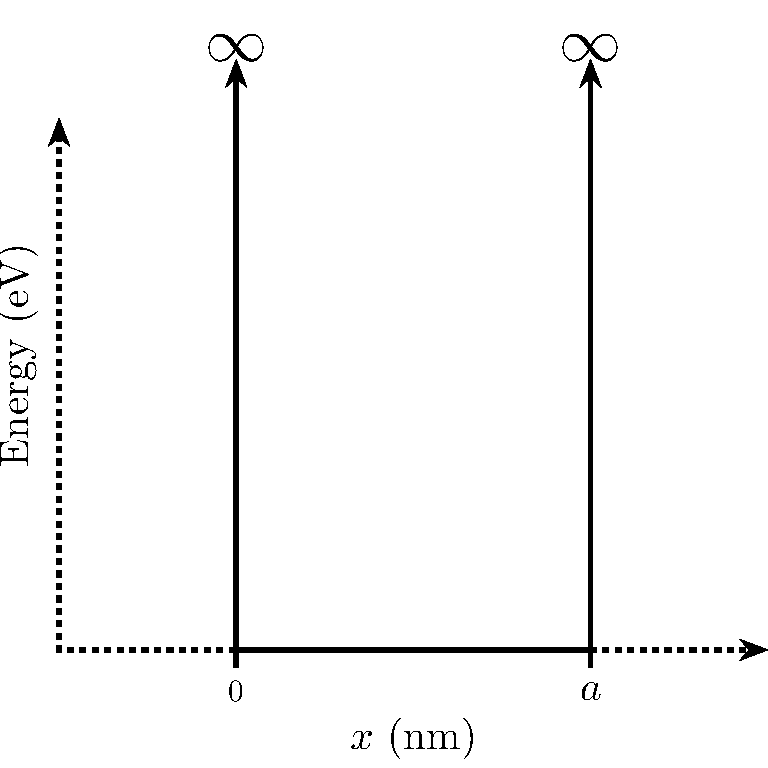
\includegraphics[width=0.4\textwidth]{./chapter-2/IWELL/IWELL}
%	\caption{Infinite rectangular well }
%\end{figure}

The electron has zero potential energy in the region $0<x<a$ where $a$ is the width of well, how previously comment the \sch  equation 



\subsection{Finite Difference Method}



S


\section{Structural Parameters}


%\begin{figure}
%	\centering
%	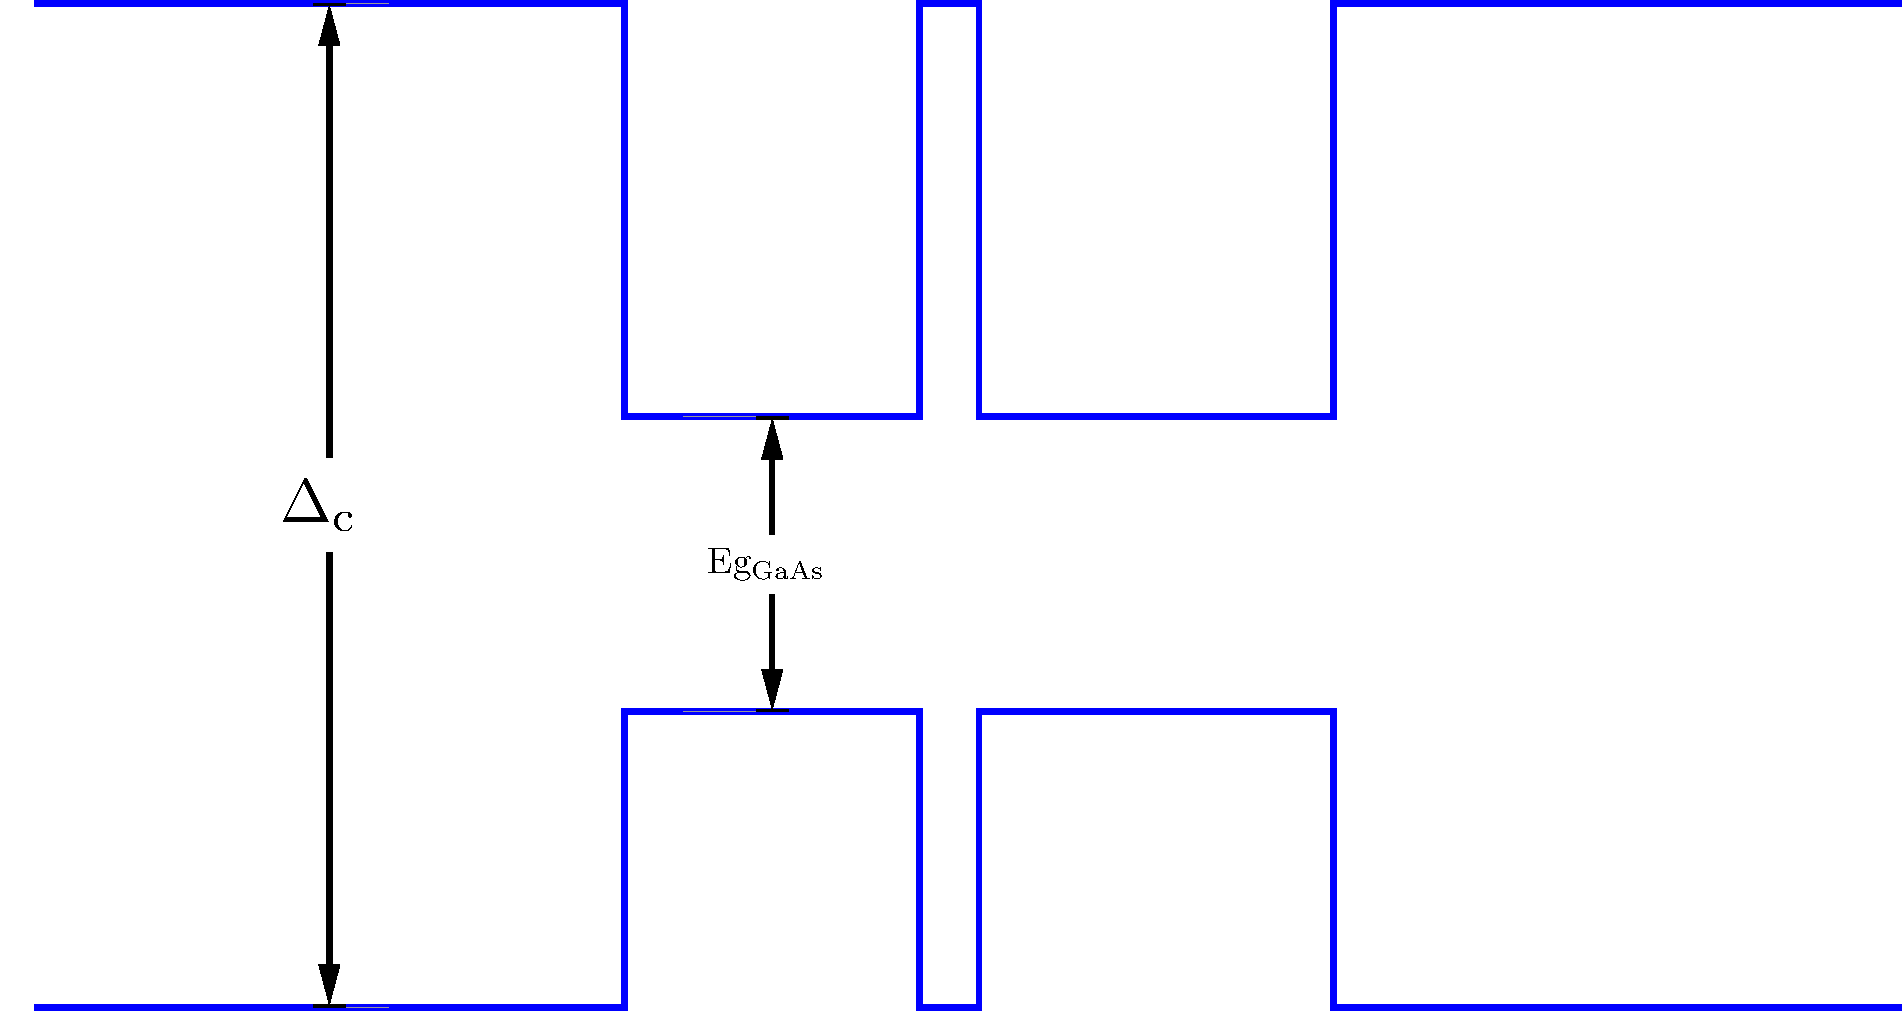
\includegraphics[width=0.3\textwidth]{./CHAPTER-3/SAMPLE-DESCRIPTION/SAMPLE-DESCRIPTION}
%	\caption{Scheme to samples }
%	\label{fig:CH2-sample-description}
%\end{figure}




\section{Anisotropy model in CQWs \label{sub:chap2-anisotropy-model}}

